\documentclass[conference]{IEEEtran}
\IEEEoverridecommandlockouts
% The preceding line is only needed to identify funding in the first footnote. If that is unneeded, please comment it out.
\usepackage{cite}
\usepackage{amsmath,amssymb,amsfonts}
%\usepackage{algorithmic}
\usepackage{algorithm2e}
\usepackage{graphicx}
\usepackage{textcomp}
\usepackage{xcolor}
\def\BibTeX{{\rm B\kern-.05em{\sc i\kern-.025em b}\kern-.08em
    T\kern-.1667em\lower.7ex\hbox{E}\kern-.125emX}}
\begin{document}

\title{Securing IoT Networks through Moving Target Defence}

\author{\IEEEauthorblockN{Andrei Vlădescu}
\IEEEauthorblockA{\textit{University POLITEHNICA of Bucharest}\\
Bucharest, Romania \\
andrei.vladescu2104@stud.acs.upb.ro}
\and
\IEEEauthorblockN{Ion Bica}
\IEEEauthorblockA{\textit{"Ferdinand I" Military Technical Academy}\\
Bucharest, Romania \\
ion.bica@mta.ro
}
}
\maketitle

\begin{abstract}
This study examines the effectiveness of Moving Target Defense (MTD) strategies in strengthening the security of Internet of Things (IoT) networks against Distributed Denial of Service (DDoS) attacks. The rapid proliferation of diverse, resource-constrained IoT devices used in every environment, ranging from smart homes to critical infrastructure has widened the gap between attackers and defenders, expanding the attack vectors and increasing network vulnerabilities. In this research, we evaluate the application of MTD techniques combined with Software-Defined Networking (SDN) to dynamically alter network configurations and disrupt attackers' strategies. 

As MTD strategies are not designed to block an attack outright, but make it costlier for the threat actor to sustain it, the described approach aims to render public IoT networks attacks logistically non-viable, thus increasing security posture. 

\end{abstract}

\begin{IEEEkeywords}
MTD, IoT, SDN, DDoS, Edge Devices
\end{IEEEkeywords}

\section{Introduction}
In recent years, the deployment of Internet of Things (IoT) devices has transformed numerous sectors, including smart homes, healthcare and critical infrastructure automation. While these devices provide efficiency and convenience, they also widen the attack vector in the cyberspace\cite{sh_xenofontos2022}. Many such edge devices operate in resource-constrained environments and often lack robust security measures or policies\cite{sh_selvaraj2023} - such as hardened applications and usage of "heavy" cryptography, making them low-hanging targets for bad actors.  
\\
In response to these security concerns, strategies such as Moving Target Defense (MTD) have emerged as a countermeasure \cite{mtd_vol1}. By dynamically altering the attack surface, MTD techniques increase the complexity and cost for the attacker, making sustained attacks less feasible. This work presents a review of relevant literature and proposes a solution tailored to the IoT security landscape, through the usage of Software Defined Networking (SDN) as a network-layer MTD strategy. 
\\
This paper analyzes the fragility of IoT  devices' services when exposed to the public Internet and tests a proxy-based strategy to hide the real IP of the protected IoT device, while also shielding it from DDoS attacks.
\\
Although this research is primarily dedicated to mitigating Distributed Denial-of-Service (DDoS) attacks, it also examines additional threat vectors within IoT environments. In particular, the proposed framework considers reconnaissance or intelligence-gathering activities, as well as more advanced exploitation attempts involving command-and-control (C2) infrastructures.
\\
The article is organized as follows: Section II introduces the context and existing work in the literature, providing a technical background on the key concepts and challenges addressed. In Section III we present the theoretical framework and mathematical models that form the foundation of our analysis. The performance of the solution is benchmarked in Section IV along with highlighting key findings.

\section{Background and Related Work}

In this section, we explore various Moving Target Defense (MTD) tactics and Software-Defined Networking (SDN) techniques discussed in the current literature. We begin by examining how an MTD strategy dynamically alters system configurations to increase uncertainty and complexity, throwing off an attacker. Subsection B is dedicated to SDN principles, how it's structured, programmed and controlled. The final subsection is dedicated to conducting a literature review.

\subsection{Moving-Target Defense}
The concept of Moving Target Defense (MTD) long predates the modern age; it may have predated written history. MTD can be described as the classical game of "shell game", in which a stone is hidden under three cups or shells, and the gambler tries to guess the location of the stone, after they were shuffled.
\\
We can define how an attack lifetime takes place by using the following formulas: 
\begin{align}
\quad & t_{\text{attack}} = t_{\text{probe}} + t_{\text{construct}} + t_{\text{launch}} \label{eq:attack_time} \\
\quad & t_0 + t_{\text{attack}} \in S_{\tau_k} \label{eq:success_condition} \\
\quad & S_{\tau_k} = [t_{\tau_k}, t_{\tau_{k+1}}) \label{eq:service_state}
\end{align}

As shown in Equation~\ref{eq:attack_time}, the attack time is the sum of the durations for probing, constructing, and launching. The successful attack condition is expressed in Equation~\ref{eq:success_condition}, as the starting time $t_0$ represents the time it took for the attack to commence during which the service was already started. The service state is defined in Equation~\ref{eq:service_state}, which refers to the state-changing nature of the MTD strategy. 

\\
Moving target defenses have been proposed as a way to make it much more difficult for an attacker to exploit a vulnerable system by changing aspects of that system to present attackers with a varying attack surface\cite{mtd_vol1}. The goal of a diverse defense is to make the attack target unpredictable, causing difficulties in delivering a malicious packet. Such strategies are already applied in a computer, such as Address Space Layout Randomization (ASLR) \cite{shacham2004}, Instruction Set Randomization (ISR) \cite{kc2003}, Honeypots (decoy nodes) or Honeynets (decoy networks). As such, different parameters can be varied so that the attacker will either miss his target, or worse, hit a decoy target.

\subsection{Software-Defined Networking}
Software-Defined Networking is a network architecture that virtualizes the network, modifying the existing conventional architecture by using a single control plane for all the data planes, instead of a one-to-one relationship. The SDN controller is the logical entity that enables network administrators to manage and dictate how the data planes, meaning switches and routers, should handle the network traffic\cite{CiscoCCNA3}.
\\
An Application Programming Interface (API) is a set of standard procedures that defines the proper way of interfacing between services of an application. The SDN controller uses northbound APIs to communicate with the upstream applications, while the southbound APIs are used in defining the behavior of the data planes.
\\

\subsection{Related Work}
% Categorize MTD into events, what they defend, etc
Early research based on random mutations \cite{al_shaer2013}\cite{jafarian2012} require each move in the random mutation takes place either at predetermined periodic intervals or at unpredictable random times, meaning the approach is proactive. 
% Talking about random mutations
\\
A generic concept that is implementing MTD through the usage of SDN is Mutable Networks (MUTE) \cite{mtd_vol1}, where IP addresses and ports are virtualized and are mapped to a routing table. These parameters are randomly shuffled using crypto-based functions and secret random keys to guarantee unpredictability and to synchronize global configuration. Also, the responses of the hosts are modified transparently to decrease chance of fingerprinting.
\\
Not specifically designed for protecting against DDoS attacks, MacFarland et al. \cite{macfarland2015} propose an anti-reconnaisance model. Utilizing SDN capabilities, the system incorporates a DNS server which communicates with an SDN controller. The SDN controller generates an IP mapping, and the DNS server provides the client with this potentially unique IP. NAT rules are applied to map the real MAC and IP addresses to synthetic values.
\\
Inspired by the concept of frequency hopping in the realm of electronic counter measures, a solution called TAP-based Port and Address Hopping (TPAH) \cite{luo2015} leverages the variation of layer 3 IP and layer 4 ports to counter DDoS flooding and port scanning. TPAH relies on the TAP virtual network driver, running in the user space, which implements dynamic hopping of both IP addresses and port numbers at specified intervals.
\\
Random Host Mutation (RHM) \cite{al_shaer2013} makes use of random, short-lived changes to host's IPs. The translation of IP addresses is resolved at the network edge using a special device, called MTG gateway. This is made possible by keeping a host mapping of virtual IPs and real IPs. The MT Controller is the authority which decides the interactions of one host to another, but after the session's lifetime is over, it will terminate it. Problems arise when taking into consideration the overhead caused by the frequent changes to the routing table and the address-space is oversubscribed, rendering routering table updates laggy, due to it's size.
\\
Leveraging the vast addressing space of IPv6, a scheme can be devised to make use of it, as the limitations of IPv4 are not easily attained. Such an approach is described in Moving Target IPv6 Defense (MT6D) \cite{dunlop2011}. This proactive approach periodically changes the IP addresses of both sender and receiver during an active session, while the sessions remain uninterrupted. Rotating the addresses mid-session prevents an attacker from determining that the same two hosts are communicating. Two implementations are available, one as a host-based embedding in software and the other as a gateway device. While the overhead is small, the packet loss varies with the file size, as the kernel buffers are filled. Latency was also observed, but the authors acknowledge that the solution could be implemented into a lower level language, compared to their solution written in Python. Other limitations of this solution include potential  collisions with other hosts, as address rotation is randomised or the ISP's inability to provide an IPv6 to every host.
%OF-RHM added
\\
Implementations that use SDN have been studied, and they make use of proven protocols, such as OpenFlow. One of these solutions is OpenFlow Random Host Mutation (OF-RHM) \cite{jafarian2012}, which makes use of OpenFlow switches, RHM gateways and controller. The controller is the authority that manages the virtual IP translations, and updates the switches accordingly so host end-to-end communication is achieved. This implementation is also studied and adopted in more modern contexts, using SYN flooding attacks as a key testing factor \cite{rochak2023}. In this study, OF-RHM is benchmarked with this type of DDoS attack and performance is evaluated by measuring the CPU utilization. Both these studies showcase the benefits of using OF-RHM, as it reduces substantially the CPU usage of flooding attacks. That being said, the mutation rate is proportional to the overhead caused by the solution.
\\
Another implementation utilizing OpenFlow is presented by Gudla et al. \cite{gudla2016}, which compares the implementation with and without MTD. During shuffling events, jitter rates in the non-MTD approach remain low, whereas in the MTD approach, jitter rates peak temporarily during the shuffling period. Due to congestion and network overhead, packets are dropped in the network.
\\
While some previous solutions use moving target defense strategies to shuffle the IP addresses the protected assets use, another method would be to vary the network configurations based on which identity the client uses. The variation based on client identity can be classified as "spatial mutation", while the shuffling based on time passing can be classified as "temporal mutation". A solution building upon these two methods is  devised by Jafarian et. al. \cite{jafarian2014}. Through theoretical analysis and empirical validation, they demonstrate the efectiveness of this MTD strategy in countering recoinnasance, worm propagation and advanced persistent threats (APTs).
% Talking about event-driven mutations
%\\
%Other strategies rely on events to trigger the shuffling of IPs, such as alerts or security policies.
\\
To address the problem associated with the overhead of shuffling, a low-complexity shuffling method known as SDN-oriented Cost-effective Edge-based MTD Approach (SCEMA) \cite{javadpour2022}, is prooposed. The study seeks to minimize implementation costs while maintaining or enhanching the security level. The Mininet implementation increases unpredictability, adding higher costs for attackers.

%\cite{zhou2019} - abandoned
%\cite{steinberger2018} - abandoned

\section{Proposed Model}
In this section, we describe the threat model we have considered in our work. 

\subsection{Threat Model}
In DDoS attacks, the attacker builds up a network of devices, either compromised or voluntarily participating \cite{sh_sekoia2023}, commonly known as a botnet. At a specified moment, the attacker sends a command to the botnet, directing it to execute a synchronized attack on a particular target. The attacker typically seeks the easiest point of vulnerability to exploit, such as an unprotected server within a larger system, to minimize the cost and effort of the attack \cite{javadpour2022}. Volumetric attacks are used by the botnets to overwhelm the target's computing capacity, such as TCP SYN Flood or UDP Flood.\\
The devices under test are resource-constrained, lacking firewalls, intrusion detection systems (IDS) or other access control lists (ACLs) to protect them against botnets. The attacked services are simulated on specific microcontrollers, using REST and CoAP protocols, to serve some data that an IoT might provide.\\
The backbone of the architecture is structured as such:

\begin{itemize}
    \item Master node
    \item Proxy node(s)
    \item Nest node(s)
    \item IoT devices
\end{itemize}

The master node is the equivalent SDN controller, but in addition handles DNS requests and additionally makes use of MQTT as southbound protocol communication with the proxies and Nest nodes.

\begin{figure}
    \centering
    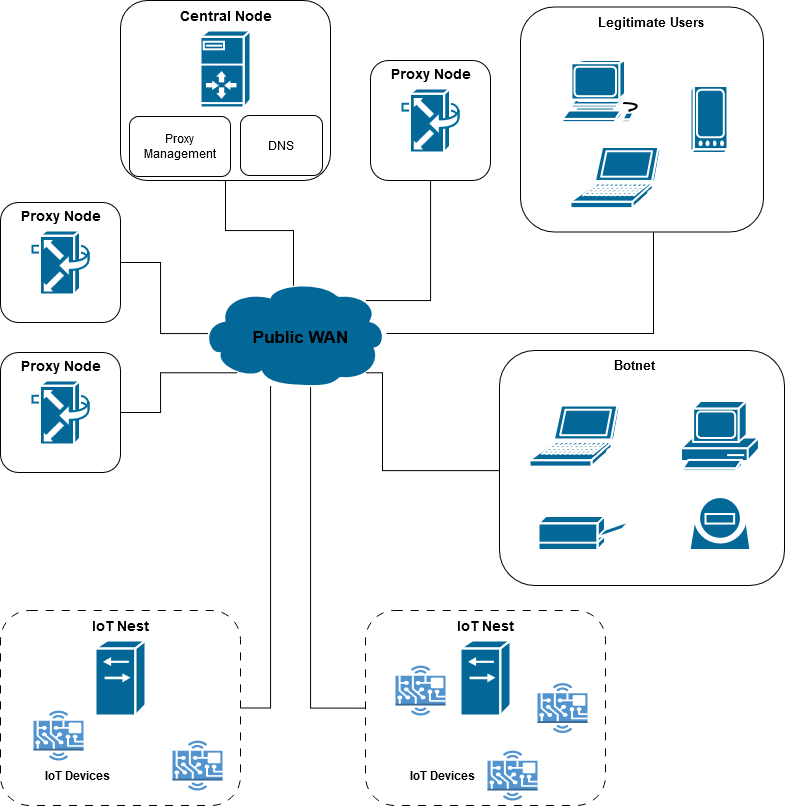
\includegraphics[width=1\linewidth]{images/architecture.png}
    \caption{System Architecture}
\end{figure}

Proxies serve as the foundational layer of abstraction, concealing the IoT nest nodes and permitting only traffic that has been independently approved by the master node. Two proxies will not have the same routing tables, as they will not have any common client-nest pairs. The access is done through nftables commands, using DNAT and SNAT.\\
Nest nodes are the final destination between the client's messages and the IoT device. They only allow traffic from a certain proxy, and serve as the gateway of the IoT LAN. In a real scenario, this gateway would have to translate any protocol from the IoT device, through any physical medium, such as Modbus over IP, in SCADA devices, or Z-Wave from a wireless sensor, thus serving as the end-goal for these non-IP appliances.
\\
The target microcontroller is a well-used Espressif ESP8266, which has been used on many smart appliances since it’s release in 2014. It has a 32bit single core Tensilica L106 running at 80 or 160 MHz, which is enough for most tasks a smart appliance may need to do, including cryptography and service hosting. 

\subsection{Infrastructure Problems and Limitations}
The primary focus is protection of IoT devices that operate without authentication, such as public infrastructure, meteorological stations, or public safety systems.
\\
The tested infrastructure operates like the public Internet, where IP translation is not feasible to rotate frequently. This is due to the Internet Service Provider's (ISP) inability to allocate a large pool of IPv4 addresses, coupled with the limited availability of IPv6 in many regions at the time of writing this paper. Proxies, master and nest nodes are all running on a docker network, the delays from the infrastructure are all minimal in this case.
\\
The IoT ecosystem in use is low-compute, meaning any disruption in service can result in infrastructure downtime, with isolated devices becoming difficult to access. This necessitates greater attention to monitoring the health of these devices, further highlighting the disparity between commercial servers and IoT devices.


\subsection{Description of the Proposed Solution}

Initial DNS resolution takes place before requesting data, and marks the beggining of the algorithm. When the client $C$ with an ephemeral IP from its ISP $C_{IP_K}$ requests the IP of the service at domain $D$, the DNS request will eventually lead to the DNS held by the architecture. This DNS is on the defender side, and works with the SDN controller to give IP addresses held by the infrastructure. \\

\begin{algorithm}
\caption{DNS Resolution with Proxy Assignment and SDN Integration}
\label{alg:dns-resolution}
\SetAlgoLined
\KwResult{Client connects to IoT Device}
\vspace{6pt}
$C_{IP_K} \xrightarrow{DNS Query} S_k$\;
\vspace{2pt}
$DNS \xrightarrow{IP_K} M_{SDN}$\;
\vspace{2pt}
\eIf{$IP_K \notin IP_{Blacklist}$}{
    \eIf{$IP_K \in \{IP_{Client} \mid (IP_K, IP_{Proxy}) \in P_{Assigned}\}$}{
        \Return{$IP_{Proxy} \mid (IP_K, IP_{Proxy}) \in P_{Assigned}$}
    }{ 
        Choose $IP_{Proxy} \sim \text{Random}(\mathcal{P})$\;
        Add $(IP_K, IP_{Proxy})$ to $P_{Assigned}$\;
        \Return{$IP_{Proxy}$}
    }
}{
    Close connection\;
}
\end{algorithm}

The end result of this algorithm is the client is returned the IP of the proxy and he can request data from it using GET requests. The designated proxy will have been modified using the southbound API by the SDN controller to allow DNAT/SNAT.\\

An attacker may not connect to the IoT device, through this infrastructure if he has not first and foremost connected each bot from his army. If he uses only the DNS from one query with all his botnet zombie devices, the DNAT/SNAT rules will not exist, and such the connection will not take place.

\begin{figure}
    \centering
    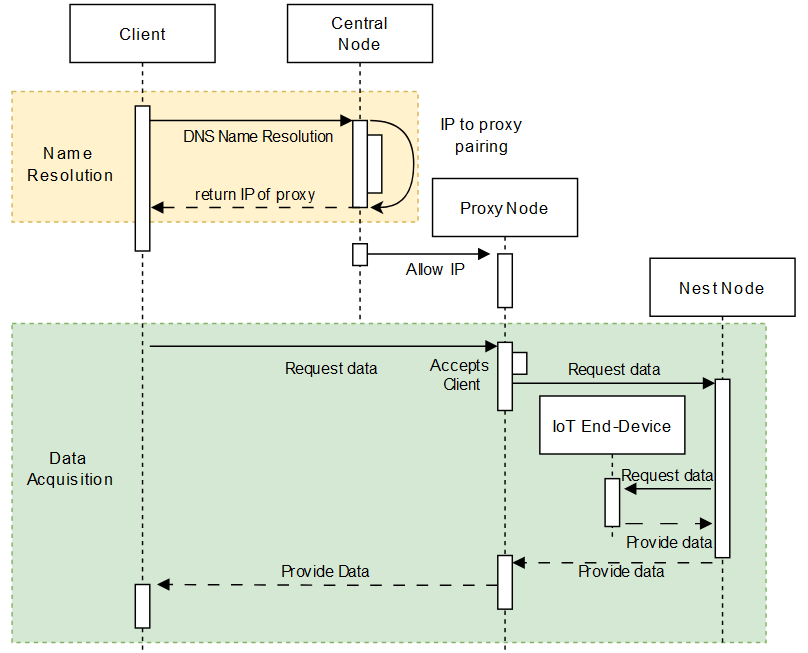
\includegraphics[width=1\linewidth]{images/sequence_diagram.png}
    \caption{Sequence Diagram of the Data Flow}
\end{figure}

After a connection takes place, the client can request data from the IoT server. He will initiate a connection to its given public proxy IP, then the proxy will masquerade the IP addresses. When the nest received the request, it relays the request to the IoT device, and the data flows back to the proxy. Source IP is again changed to reflect the source of the packets as being the proxy, $IP_{Proxy}$.

\begin{algorithm}
\caption{Client-Server Communication Dataflow}
\label{alg:data-flow}
\SetAlgoLined
\KwResult{Client retrieves data from IoT Device}
\vspace{6pt}
$C_{IP_K} \xrightarrow{\text{GET Request}} P_{IP_{Proxy}}$\;
\vspace{4pt}
\eIf{$IP_K \in P_{Allowed}$}{
    \vspace{2pt}
    $NAT(IP_K \to IP_{Proxy}, IP_{Proxy} \to IP_{Nest})$\;
    $IP_{Nest} \iff IP_{IoT}$\;
}{
    Close connection\;
}
\end{algorithm}

The DDoS detection used is volumetric, it does not take into account other more sophisticated ways a system may be DDoS-ed, however this is a different topic, as a different DDoS detection system may be implemented in place of the used one. Newer systems can be wired directly in-place of this module, piping the data flow analytics to a ML model and template matching signatures from one packet to another.\\
When a certain IoT service is under attack by a botnet, a proxy detects the large number of requests per period of testing, and will notify the master node. The master will therefore request a new IP from the ISP, through it's vendor-specific API, and inform the proxy of the change when it's done. 

\begin{algorithm}
\caption{Handling of an Attack Through Naive Detection}
\label{alg:attack-flow}
\SetAlgoLined
\KwResult{Attacker is interrupted proactively}
\vspace{6pt}
\While{Proxy Server Active}{
\State $R \gets \frac{N_{req}(T)}{T}$ \;
\vspace{4pt}
        \If{$R > R_{th}$}{
        \State $ M_{SDN} \xleftarrow[Renew IP]{\text{DDoS Attempt}}Proxy$\;
        \vspace{6pt}
        \State $M_{SDN} \xrightarrow[Provider API]{\text{Request new IP}} ISP$ \;
        \vspace{6pt}
        \State $IP_{Proxy_{Old}} \xleftarrow{\text{Replace}} IP_{Proxy_{New}}$
    }
    \EndIf
}
\EndWhile{}
\end{algorithm}


\section{Evaluation}
In this section we evaluate the performance of the proposed solution in terms of its effectiveness in mitigating attacks from botnets. % Communication between clients and the IoT service being provided is also taken into account, to create a baseline evaluation of how it should work.
\subsection{Evaluation Metrics}
The primary objectives are to lower defense costs for the defender and maintain reliable service for clients. To assess the achievement of these goals, the following metrics must be evaluated:
\subsubsection{Delay Times}
Delay time refers to the time taken for a request to travel from a client to the server and back. It can also be referred to as latency. \\
Delay time plays an important role in evaluating the usability of a service, as prolonged delays can render the service unattractive, regardless of its level of security. These delays are measured using Locust and Requests libraries in Python.
\subsubsection{Failure Rate}
Failure rate is another very important aspect for the client side, as a high failure rate can make the service unusable. This metric is assessed under normal usage conditions as well as during an attack.
\subsubsection{Power Usage}
Since many IoT devices are designed to operate on battery power rather than being connected to the grid, power consumption becomes an important factor to take into consideration. This may determine whether a device functions for two years or just two months. Frequent maintenance and battery replacements not only cause inconvenience but also lead to higher operating costs. Power usage is measured using a 5-digit laboratory power supply.

\subsection{Simulation Environment}
The network and its services have been simulated using Docker Network, with routes configured to the host network where the IoT device resides. The clients, proxies, nest, and master node are each deployed in separate containers and connected through the bridge interface of the Docker network.\\

The simulation scenarios are branched into three distinct categories:
\begin{itemize}
    \item No clients connecting to the service, establishing an anti-bias baseline.
    \item Nominal network usage, where a maximum of 10 requests per second are recorded.
    \item A botnet volumetric attack, simulating a high request rate per second (RPS) from lots of clients. 
\end{itemize}

%The simulation time allocated for each scenario is 100 seconds.

\subsection{Simulation Benchmark}
The obtained results of each discussed metric are presented in this subsection. \\


\subsubsection*{Delay Times Results}
In normal usage of the microservice, the statistics from Fig. \ref{fig:nominal-statistics} are relevant. The requests per second (RPS) metric is above 3, after all users have connected and started communicating with the IoT device. These kind of RPS are situated on the border of acceptable, from the standpoint of volumetric attacks threshold set for this solution.
\\
A response time of 60ms is observed when no outliers are considered, with no more than 150ms latency to be expected, well within the margin of acceptable server delay.
\\
Considering a normal baseline, in Fig. \ref{fig:ddos-statistics} the statistics show a different story. Users are ramping by 100 at a time, introducing a big latency, of 20s (capped by Locust). The 95th percentile statistic is in the outlier, showing what a minority of users might encounter, while 50th percentile describes what a normal user will see when connecting to the microservice, while it's under heavy (DDoS) load. 

% Urmeaza statisticile unde sistemul este protejat de algoritm 
\begin{figure}
    \centering
    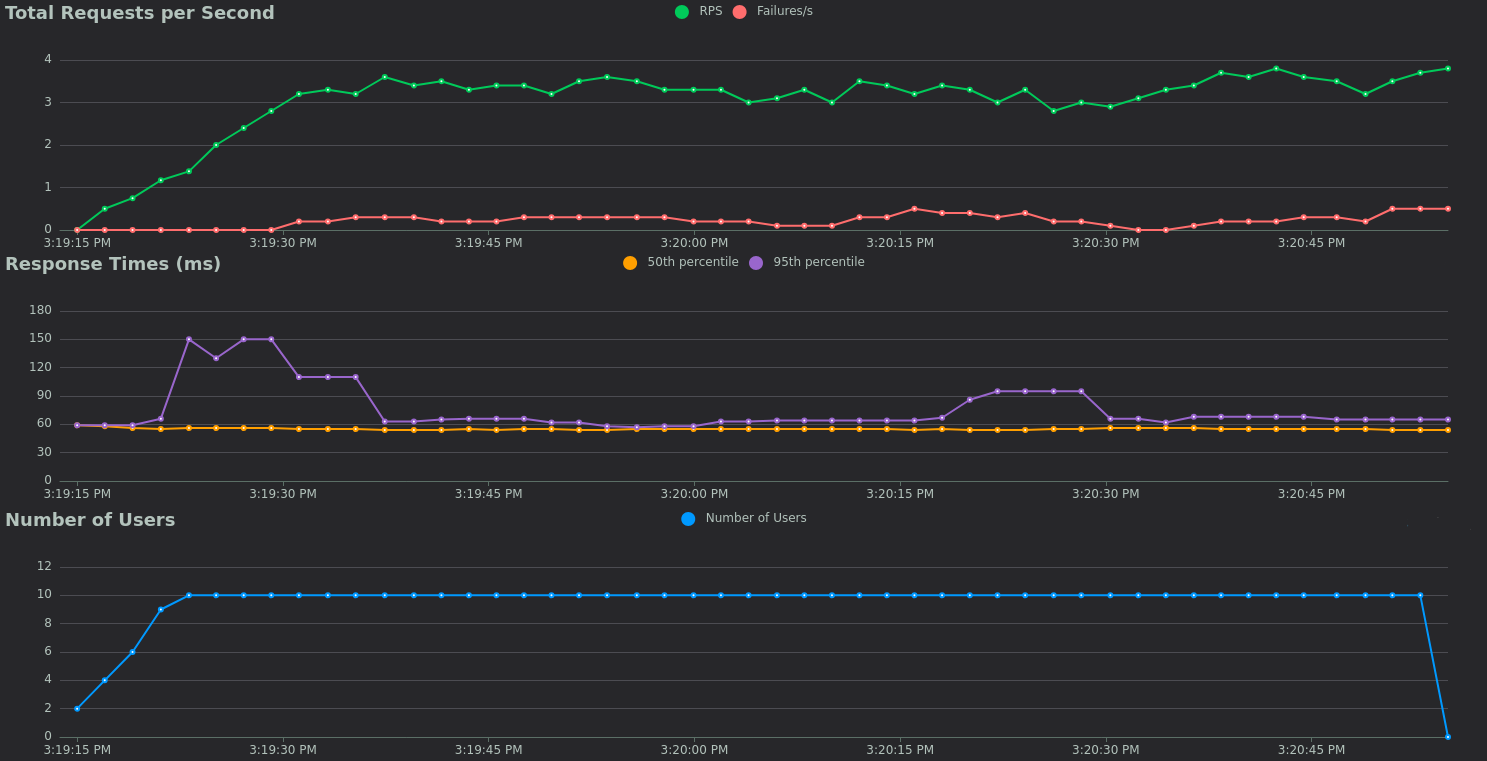
\includegraphics[width=1\linewidth]{images/nominal_usage.png}
    \caption{Locust Nominal Statistics}
    \label{fig:nominal-statistics}
\end{figure}

\begin{figure}
    \centering
    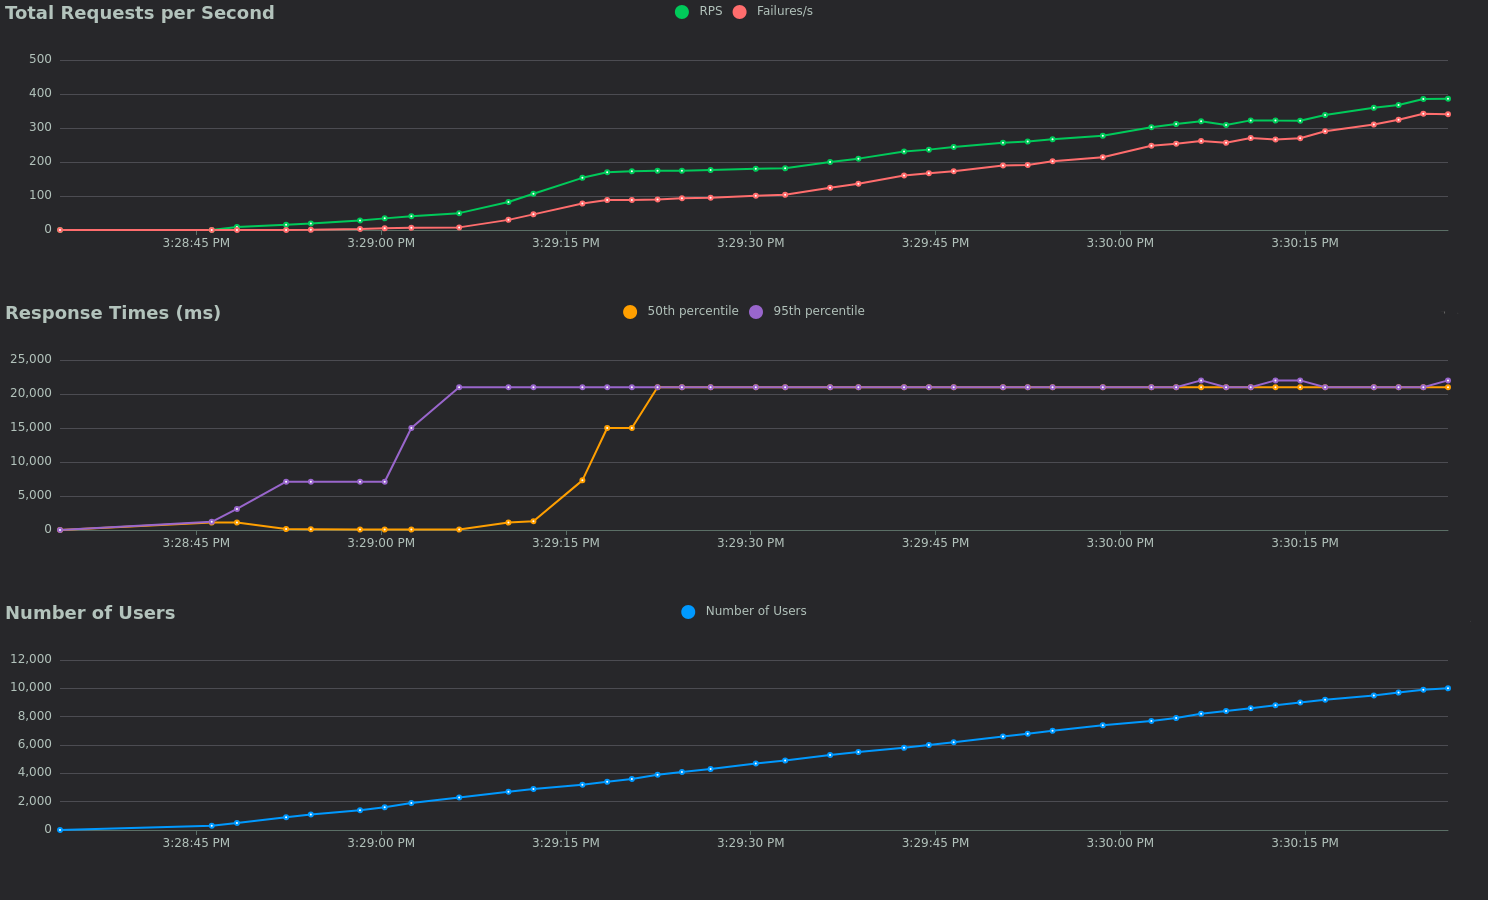
\includegraphics[width=1\linewidth]{images/ddos_usage.png}
    \caption{Locust Unprotected DDoS Statistics}
    \label{fig:ddos-statistics}
\end{figure}

\subsubsection*{Failure Rate Results}
Failure rate under nominal load is displayed in Fig. \ref{fig:nominal-statistics}. A fractionary rate of failures/s can be explained by taking into account how Locust averages failures over a window of time, rather than counting them as a whole number every second. These low rates are happening when taking into consideration even low RPS, of around 3, showcasing the need for robust mechanisms for caching, if available.
\\
Under a heavy load, the failure rate grows directly proportional to the RPS, as the server will never be able to handle all the requests.

\subsubsection*{Power Usage Results}

When analyzing the power draw of this embedded device, it is important to note that no power optimizations, such as microcontroller deep sleep or caching mechanisms are being used. Raw power usage is bigger in our case, as for each request a SHA512 will be completed along with a temperature read, as to simulate a non-trivial computational load that an IoT microservice might encounter.
\\
To simulate the DDoS under a realistic scenario, a Ixia PerfectStorm ONE packet generator appliance has been used. A HTTP DDoS scenario has been orchestrated with a throughput of 1 GBps. A full 10.10.0.0/16 network segment has been reserved for this attack.

\begin{figure}
    \centering
    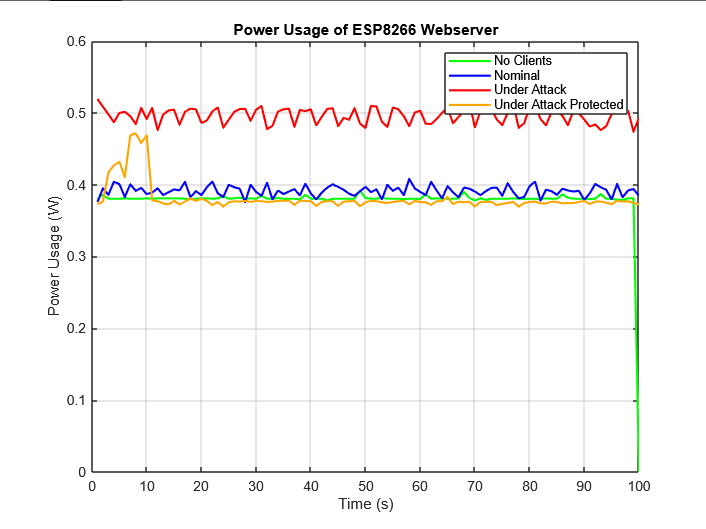
\includegraphics[width=1\linewidth]{images/power_usage_esp8266.png}
    \caption{Power Usage of ESP8266 Webserver in Different Scenarios}
    \label{fig:power-usage}
\end{figure}

As shown in Fig. \ref{fig:power-usage}, under a DDoS load the webserver draws a lot more power, peaking at more than 165\% compared to nominal load. In terms of battery usage, if a battery would be depleted in a year, under significant load it would not exceed 7 months - time in which the service is not consistently usable.
\\
In the realistic scenario, the packet generator has been configured with a loading curve \ref{fig:data-rate}. The attack took 100 seconds in the full loading phase, with a 2-second loading phase. The orange curve in Fig. \ref{fig:power-usage} describes the behaviour of the system; in a 10 second time window the attack has been stopped entirely. The peaks shown in the unprotected scenario are higher, compared to the orange curve, meaning the system managed to stop the DDoS attack faster than it had attacked the ESP web server, since the power curve shows the average load per second.
\\
\begin{figure}
    \centering
    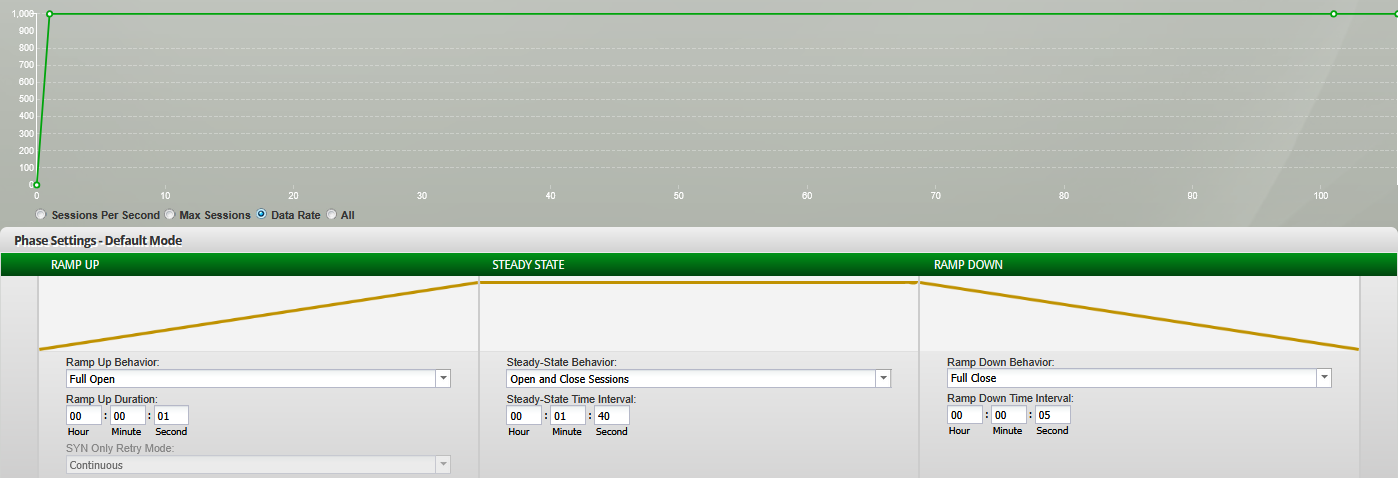
\includegraphics[width=1.03\linewidth]{images/breakingpoint_curve.png}
    \caption{Ixia Packet Generator Data Rate Curve}
    \label{fig:data-rate}
\end{figure}

\section{Acknowledgements}
This work was supported by a grant of the Ministry of Research, Innovation and Digitization, CCCDI - UEFISCDI, project number PN-IV-P6-6.3-SOL-2024-0279, within PNCDI IV.

\bibliographystyle{IEEEtran}
\bibliography{references} % Replace 'references' with the name of your .bib file, without the .bib extension.

\vspace{12pt}

\end{document}
